\documentclass{article}
\input{boilerplate}
\author{}
\setlength{\headheight}{28pt}

\begin{document}


\newcommand{\lectureTitle}{Generalizable RL for Neighborhood Battery Control in CityLearn}
\newcommand{\lectureDate}{Due: May 8th, 23:59}

\textsc{COS435 / ECE433: Introduction to RL}
\vspace{1em} \hfill \lectureDate

\maketitle
\setlength{\headheight}{28pt}

\paragraph{Authors.} Grace Sun (\texttt{gs0625@princeton.edu}), Ammaar Alam (\texttt{ah0952@princeton.edu}), Erik Dyer (\texttt{ed1783@princeton.edu})

\paragraph{Link to GitHub Repo.} \url{https://github.com/Ammaar-Alam/cos435-citylearn}

\section{Introduction}

Buildings account for approximately 28\% of global CO$_2$ emissions \citep{iea2022buildings}, so coordinating distributed energy resources such as solar PV and battery storage is a control problem with real-world stakes. Batteries can absorb excess solar power, reduce peak demand, and shift consumption away from high-carbon hours, making building energy management a natural testbed for reinforcement learning: actions have delayed consequences, rewards combine several objectives, and policies must generalize beyond the data they see during training.

The CityLearn Challenge 2023 \citep{citylearn2023} formalizes this as a sequential decision-making benchmark. At each hourly timestep, a controller observes building-level variables such as solar generation, net electricity demand, battery charge, temperature, and short-horizon forecasts, then emits one continuous charge/discharge action $a_t \in [-1,+1]$ per building. The final score combines five normalized KPIs: electricity cost, carbon emissions, daily peak demand, thermal discomfort, and thermal resilience loss. A strong controller must therefore decide when to reserve battery capacity, when to prioritize cost or carbon, and how to avoid improving one KPI at the expense of another.

The main challenge is generalization. A learned policy can overfit to a training split, and a centralized policy whose input and output layers are fixed to three buildings cannot run on a six-building neighborhood. Rule-based control (RBC) avoids these failure modes by encoding human priors rather than fitting data, which helps explain why strong CityLearn entries such as CHESCA \citep{pinto2024citylearn} have favored hierarchical optimization over learned policies. Prior RL approaches to CityLearn have struggled with three recurring gaps: rewards often do not match the composite evaluation criterion, single-run results overstate reliability, and fixed-topology architectures cannot adapt to neighborhoods of different sizes.

We ask whether a systematic RL pipeline can outperform RBC on held-out evaluation data while remaining portable to building configurations unseen during training. We run a controlled ablation across two algorithms (PPO and SAC), two control topologies (centralized and shared-parameter decentralized), and three reward variants, using multiseed runs ($n = 3$--$10$) and confidence intervals. We then extend the shared-controller study with PPO/SAC/TD3 sweeps on Princeton Neuronic to test whether the same conclusions survive broader seed, learning-rate, and algorithm coverage. Section~\ref{sec:related} reviews related work; Section~\ref{sec:methods} describes the experimental design; Section~\ref{sec:results} presents results; and Section~\ref{sec:discussion} discusses findings and limitations. Our main contributions are

\begin{itemize}
    \item SAC with a reward aligned to the official scoring terms reduces the RBC composite score by 48.4\% on the local evaluation dataset and by 40\% on the released held-out phase-2 splits. For the fixed 3-building phase-2 setting, deterministic mean-action ensembles of centralized SAC checkpoints further reduce the SAC-family phase-2 mean to 0.616, though these ensembles are not portable to 6-building phase-3 splits.
    \item Shared-parameter decentralized training/execution (shared-DTDE) is the only topology portable to the 6-building phase-3 held-out splits; among portable policies, SAC-DTDE outperforms PPO-DTDE on phase-3 (0.774 vs.\ 0.843).
    \item A reward design ablation shows that matching the official scoring terms improves local performance, while adding battery smoothness penalties improves held-out phase-2 generalization.
    \item The final shared-controller sweep adds TD3 as a stretch algorithm. SAC remains the strongest learned controller overall in the targeted matrix (0.702 released-all), while TD3 is competitive and gives the best broad-sweep phase-3 score (0.736).
\end{itemize}

\section{Related Work}\label{sec:related}

CityLearn \citep{vazquez2020citylearn, citylearnrepo} has been used in several competition tracks on building-level energy management. The strongest 2023 entries combined forecasting, hierarchy, and optimization rather than end-to-end learned control. CHESCA \citep{pinto2024citylearn} optimized individual building behavior and then refined decisions with a community-level controller. The second-place solution \citep{zheng2025optimizing} combined learned forecasts with building-level and microgrid-level model predictive control, and earlier competition work also found online optimization to be highly competitive \citep{khattar2023winning}. These results motivate our narrower question: which RL design choices make a simple learned controller credible, reproducible, and portable, and how much of the gap to optimization can they close?

Our original ablation evaluates PPO \citep{schulman2017proximal} and SAC \citep{haarnoja2018soft}, and the final sweep adds TD3 \citep{fujimoto2018addressing}. PPO is an on-policy method with a clipped surrogate objective that stabilizes policy-gradient updates. SAC is an off-policy actor-critic method with entropy regularization and replay, which is useful in sample-limited continuous control. TD3 is an off-policy deterministic actor-critic method with twin critics, delayed policy updates, and target policy smoothing to reduce overestimation. CityLearn makes these algorithms difficult to compare because episodes span a full year of hourly control, KPI terms operate on different timescales, and battery actions have delayed effects. These properties motivate both off-policy baselines and a reward-design ablation that directly tests alignment between the training signal and the evaluation score.

Centralized versus decentralized control has also been studied directly for building energy management. \citet{kathirgamanathan2021centralised} compared centralized and decentralized RL for smart-grid battery control and found tradeoffs between coordination quality and scalability. Centralized policies can optimize a joint action but do not generalize to different numbers of buildings. Shared-parameter decentralized policies treat buildings as repeated instances of the same local control problem, so a single checkpoint can run on any neighborhood size. We extend this comparison by evaluating topology tradeoffs across same-size and cross-size held-out splits under a systematic reward ablation.

\section{Methods}\label{sec:methods}

We compare two RL algorithms across two control topologies and three reward formulations, evaluated on local and released held-out splits from the CityLearn 2023 competition. We then add TD3 and larger shared-controller sweeps so that the final claims are not based only on the earlier pilot matrix.

\paragraph{Environment.} We use the CityLearn Gymnasium environment \citep{vazquez2020citylearn, citylearnrepo} in its 2023 competition configuration of a 3-building neighborhood with rooftop solar PV and battery storage at each building. Observations include time-of-day encodings, normalized net electricity demand, solar generation, battery state of charge, and short-horizon forecasts. The composite score (lower is better) is a normalized weighted average of five KPI ratios, each comparing agent performance to a do-nothing baseline.

\paragraph{Control topologies.} We evaluate two architectures. In the centralized topology, one neural network receives the concatenated observations of all three buildings and emits a three-dimensional joint action. This gives the policy full neighborhood information but fixes the network dimensions to the training building count. In the shared-DTDE topology, one policy network is applied independently to each building's local observation window. Buildings act without observing one another at inference time, while training reuses experience across buildings through shared parameters and, for SAC, a shared replay buffer. Because the policy is applied per building, the same checkpoint runs on any number of buildings by making $N$ independent forward passes.

\paragraph{Algorithms and architecture.}
\begin{itemize}
    \item PPO \citep{schulman2017proximal}: on-policy proximal policy optimization with a clipped surrogate objective. We implement centralized PPO with Stable-Baselines3 \citep{raffin2021stable} and a custom shared-DTDE variant with per-building embeddings. The shared-DTDE PPO policy uses a 2-layer MLP (256 hidden units per layer) applied per building; the rollout buffer pools experience across all buildings. We sweep learning rates over $\{10^{-4}, 3\times10^{-4}\}$ across 10 seeds.
    \item SAC \citep{haarnoja2018soft}: off-policy soft actor-critic with entropy regularization. SAC reuses transitions through replay, which is useful in sample-limited continuous control settings. Both the centralized and shared-DTDE SAC variants use 2-layer MLP actor and critic networks (256 hidden units), a replay buffer of size $10^6$, and automatic entropy tuning. We implement centralized SAC (5 seeds) and a shared-DTDE SAC pilot (3 seeds), the latter using a shared replay buffer that pools transitions from all buildings.
    \item TD3 \citep{fujimoto2018addressing}: off-policy deterministic actor-critic with twin critics, target networks, target policy smoothing, delayed actor updates, replay normalization, and deterministic evaluation. We use TD3 as a stretch shared-DTDE algorithm in the final sweeps, using the same count-invariant shared district context features as the shared SAC controller.
\end{itemize}

All policies train for either 500K or 1M environment steps. Centralized policies treat the 3-building tuple as a single environment step; shared-DTDE variants accumulate one transition per building per environment step, effectively multiplying the transition count by the number of buildings. Checkpoints are saved every 50K steps and the final checkpoint (not the best validation checkpoint) is used for evaluation, which avoids implicit validation leakage.

\paragraph{Final shared-controller sweeps.} After the initial ablation, we ran two larger shared-controller sweeps on Princeton Neuronic. The broad learning-rate screen contains 504 summary rows: PPO/SAC/TD3 $\times$ 8 learning rates $\times$ 3 seeds, evaluated on \texttt{public\_dev}, three released phase-2 splits, and three released phase-3 splits. The targeted final sweep contains 567 rows with algorithm-specific hyperparameters: entropy coefficient for PPO, reward scaling for SAC, and exploration noise for TD3. The repository records the selected settings and aggregate results for each algorithm/evaluation group.

\paragraph{SAC checkpoint ensembles.} For same-topology phase-2 evaluation, we also evaluate deterministic mean-action ensembles of saved centralized SAC checkpoints. At each timestep, each member checkpoint proposes a continuous battery action vector; the ensemble averages those actions componentwise and clips the result to the environment action bounds. The ensemble family includes all-central checkpoint averaging, baseline-only averaging, weighted public-dev-selected members, temporal-bootstrap selection, and critic-guided local action refinement. These variants are reported only for 3-building phase-2 splits because the centralized checkpoints have fixed input and output dimensions, so we treat them as same-topology ablations rather than portable-controller results.

\paragraph{Reward design.} The default CityLearn reward is a negative net consumption proxy, but the competition ranks submissions using a multi-term composite score. We test three reward variants:

\begin{itemize}
    \item \texttt{reward\_v0} (baseline): the environment's built-in default reward. This is a sanity check because the training signal does not directly match the evaluation criterion.
    \item \texttt{reward\_v1}: a handcrafted 8-term weighted penalty mirroring the official 2023 scoring formula. Component weights are thermal discomfort ($0.30$), outage discomfort ($0.15$), unserved energy ($0.15$), carbon emissions ($0.10$), and four peak/ramping terms at $0.075$ each.
    \item \texttt{reward\_v2}: extends \texttt{reward\_v1} with two battery smoothness penalties: an SoC-change penalty ($0.05 \cdot |\Delta \text{SoC}|$) and a binary charge-to-discharge sign-flip penalty ($0.05 \cdot \mathbf{1}[\text{sign flip}]$). These terms discourage control that exploits the training split but generalizes poorly.
\end{itemize}

The reward variant ablation is fully crossed for centralized SAC. PPO uses \texttt{reward\_v2} throughout because of compute constraints.

\paragraph{Evaluation protocol.} We evaluate in three regimes. Local \texttt{public\_dev} is our primary tuning environment (one 3-building dataset available during development). Released phase-2 online-eval contains three held-out 3-building datasets, testing same-topology generalization. Released phase-3 contains three held-out 6-building datasets, testing cross-size generalization. Only shared-DTDE policies can run on phase-3. We report seed-averaged means with 95\% confidence intervals. For single-split results, intervals are over seeds; for aggregate held-out results, intervals are over seed $\times$ split evaluation jobs unless otherwise noted. A stricter protocol would cluster by split, so these intervals should be read as job-level uncertainty rather than fully independent split-level uncertainty.

\paragraph{Implementation and reproducibility.} All reported numbers come from saved checkpoints evaluated against named split configs, not last-step training scores. Aggregation scripts write the tables and figures from recorded evaluation summaries in \texttt{submission/results/} and \texttt{submission/figures/}. The ensemble and optimization-context summaries are tracked as compact CSVs in \texttt{submission/results/}. Seed counts are reported in the relevant tables; for example, the SAC-DTDE pilot is labeled as a 3-seed run.

\section{Results}\label{sec:results}

We organize results around local tuning performance, same-topology held-out generalization during phase-2, and cross-size generalization during phase-3. Figures and tables report seed-averaged means with 95\% confidence intervals unless otherwise noted.

\paragraph{Final shared-controller sweep.} The original ablation below compares PPO and SAC under the reward and topology design choices developed during the project. After adding TD3 and running the larger shared-controller sweeps, the learned-controller ordering remains SAC first, TD3 close behind, and PPO weaker. In the targeted final sweep, SAC achieves the best released-all learned score at $0.702 \pm 0.023$, followed by TD3 at $0.727 \pm 0.017$ and PPO at $0.799 \pm 0.018$. The same table keeps the RBC reference visible, showing that every learned shared controller improves over RBC while still trailing the CHESCA optimization reference on released phase-2.

\begin{figure}[ht]
    \centering
    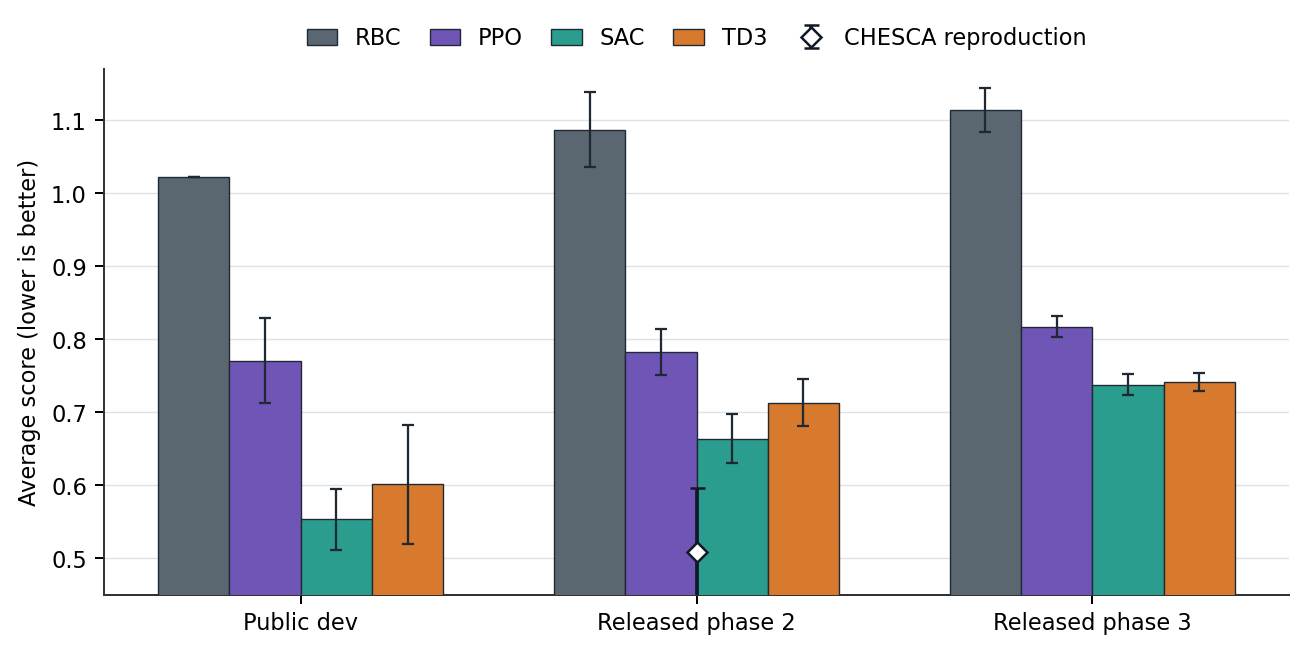
\includegraphics[width=\linewidth]{figures/final_result_matrix.png}
    \caption{Targeted PPO/SAC/TD3 shared-controller sweep. Bars show the best setting per learned algorithm and evaluation group; error bars are 95\% confidence intervals over evaluation jobs. CHESCA is an optimization reference.}
    \label{fig:final_matrix}
\end{figure}

\begin{table}[ht]
\centering
\small
\begin{tabular}{lcccc}
\toprule
\textbf{Algorithm} & \textbf{Public dev} & \textbf{Phase-2} & \textbf{Phase-3} & \textbf{Released all} \\
\midrule
RBC & 1.023 & 1.087 & 1.114 & 1.100 \\
PPO & 0.771 & 0.782 & 0.817 & 0.799 \\
SAC & 0.553 & 0.664 & 0.738 & 0.702 \\
TD3 & 0.601 & 0.713 & 0.742 & 0.727 \\
\bottomrule
\end{tabular}
\caption{Best shared-controller scores from the targeted sweep. Each learned-method cell selects that algorithm's best setting for the evaluation group.}
\label{tab:final_matrix}
\end{table}

\paragraph{TD3 stretch result.} TD3 was added as a compute-heavy stretch algorithm to test whether deterministic off-policy control could improve cross-topology transfer. The broad learning-rate screen gives its strongest result: TD3 with learning rate $3{\times}10^{-4}$ achieves $0.736 \pm 0.020$ on the released phase-3 splits, just ahead of SAC at $0.738 \pm 0.008$. In the targeted final sweep, SAC slightly retakes the phase-3 lead ($0.738$ versus $0.742$), but TD3 remains competitive and beats PPO by roughly 0.075 absolute score units on the released phase-3 splits.

\begin{figure}[ht]
    \centering
    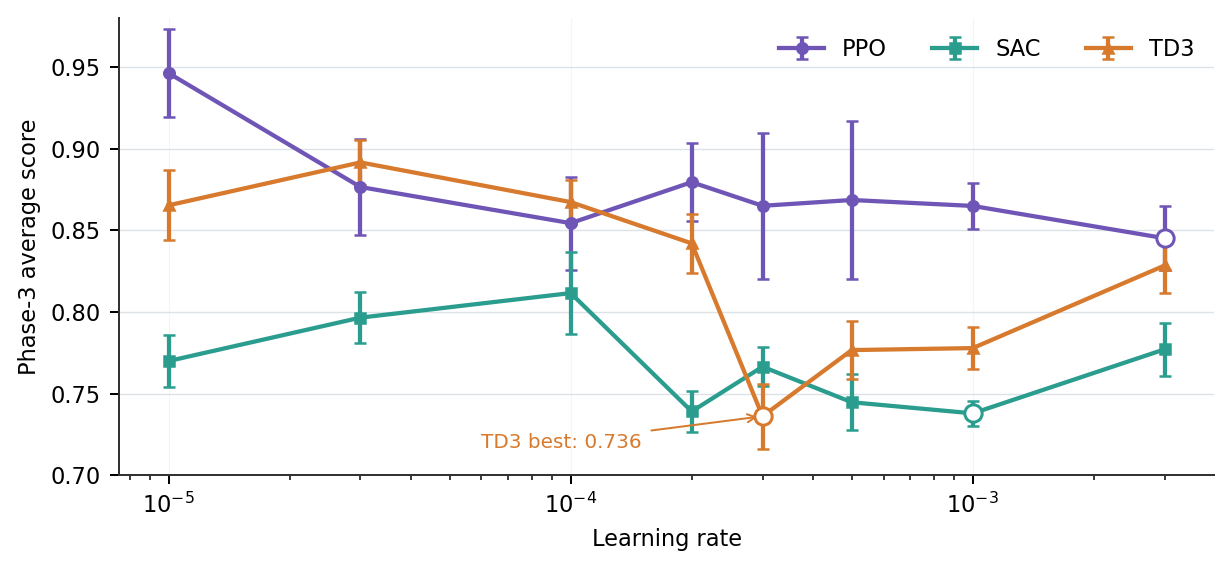
\includegraphics[width=0.92\linewidth]{figures/lr_screen_phase3.png}
    \caption{Broad learning-rate screen on released phase-3 transfer splits. Each point aggregates three seeds over three 6-building splits; TD3 peaks at $3{\times}10^{-4}$.}
    \label{fig:lr_phase3}
\end{figure}

\begin{figure}[t]
    \centering
    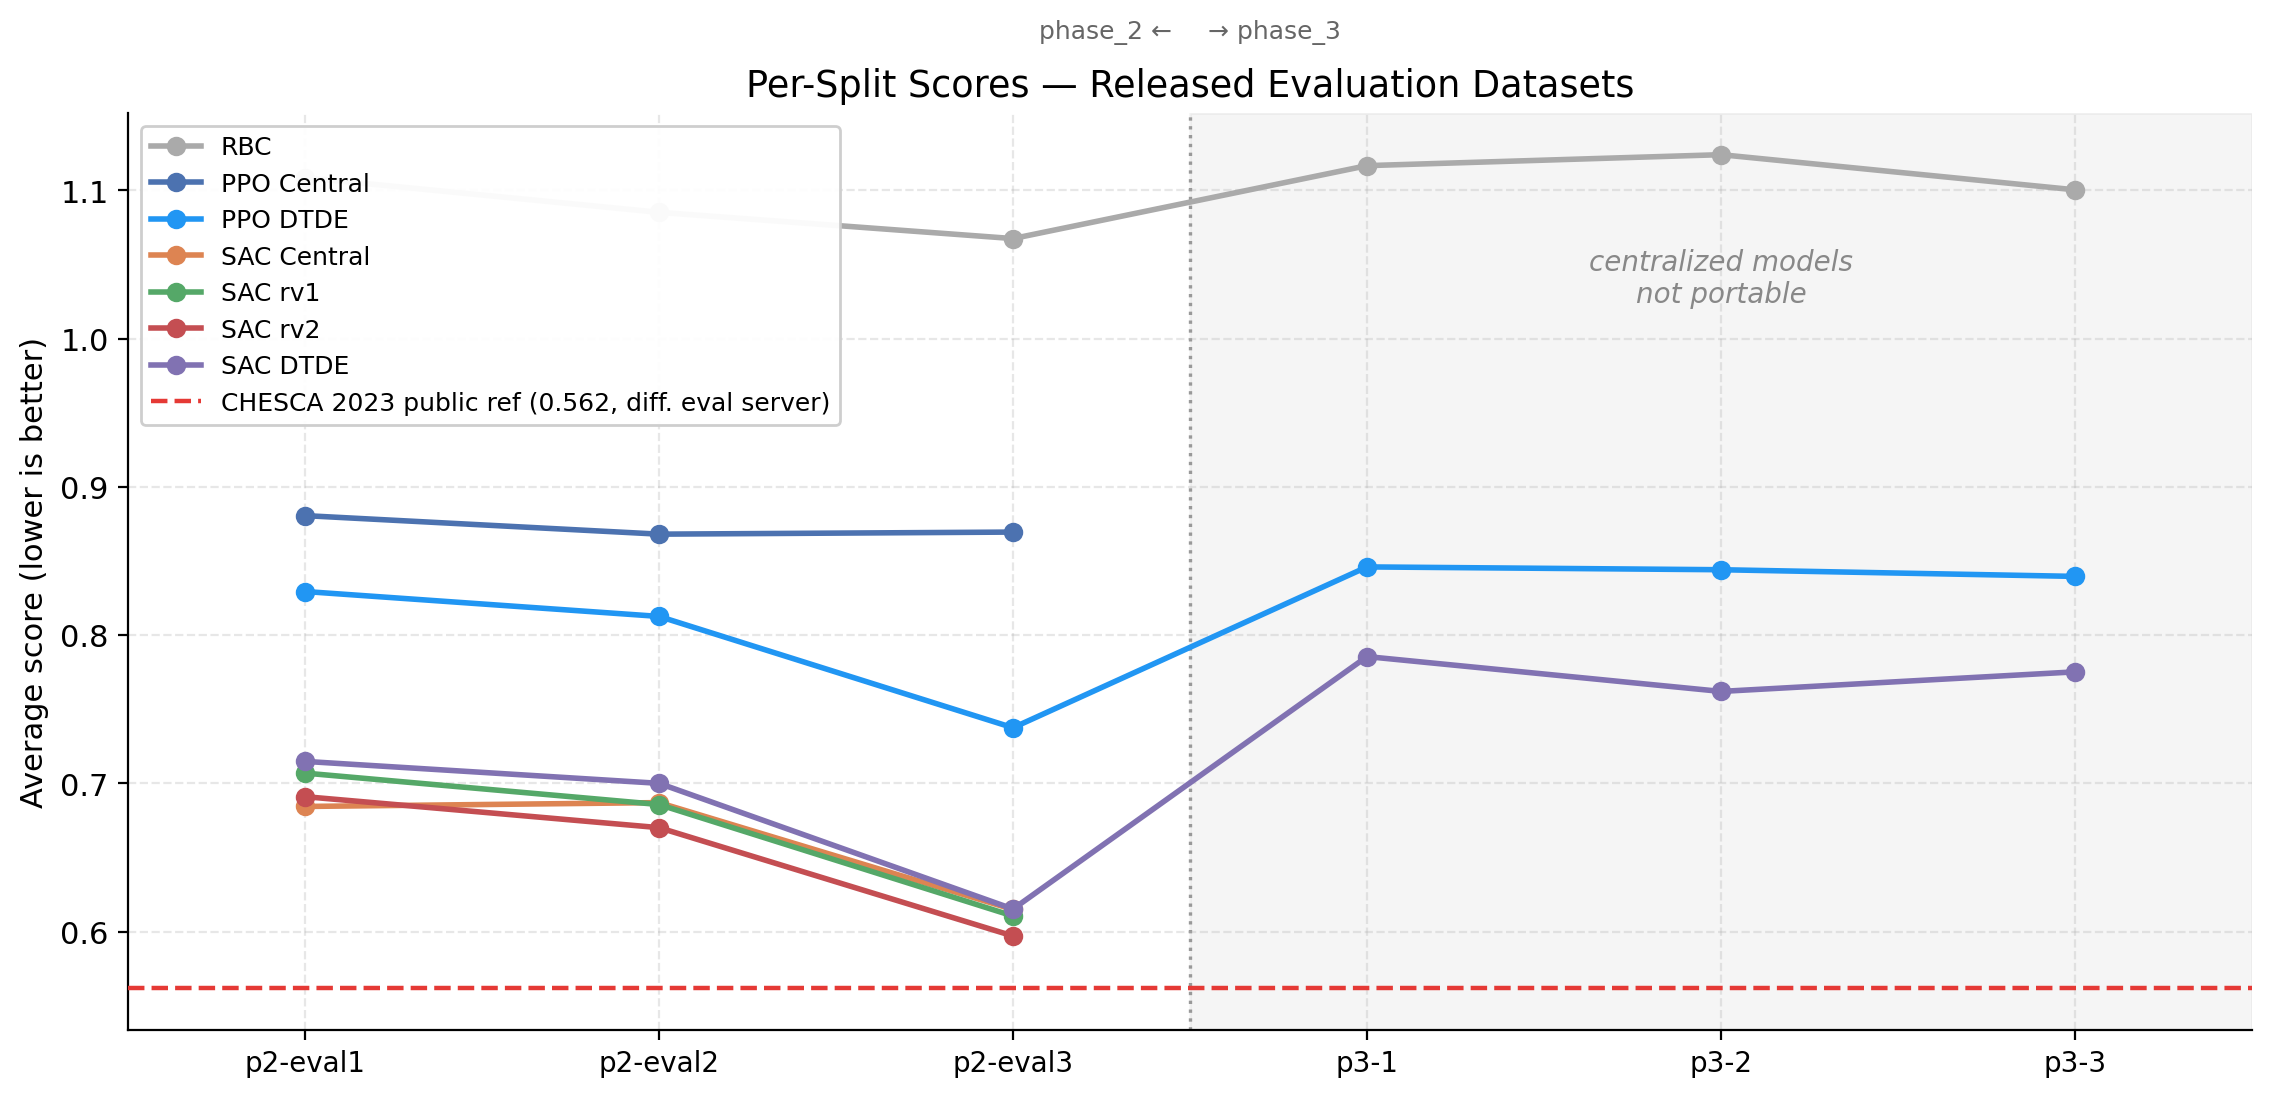
\includegraphics[width=\linewidth]{figures/per_split_scores.png}
    \caption{Released held-out scores across phase-2 (3 buildings) and phase-3 (6 buildings). Centralized policies cannot run on phase-3; SAC-DTDE is the best portable phase-3 policy. The dashed line is the CHESCA 2023 leaderboard reference.}
    \label{fig:per_split}
\end{figure}

\paragraph{Local evaluation.} Table~\ref{tab:local} summarizes results on the local \texttt{public\_dev} split. The local RBC baseline scores 1.023, and every RL method improves on it. The best local variant is SAC centralized \texttt{reward\_v1} at $0.527 \pm 0.011$ (5 seeds), a 48.4\% reduction relative to RBC. SAC \texttt{reward\_v2} ($0.536 \pm 0.016$) and the SAC baseline ($0.554 \pm 0.009$) trail by 0.009--0.027 absolute score units, indicating that reward alignment helps but is not the sole driver. SAC shared-DTDE scores $0.569 \pm 0.018$ (3-seed pilot), modestly behind centralized SAC. The decentralized controller sees only per-building observations and cannot jointly coordinate charge/discharge across the neighborhood. PPO variants are substantially weaker (0.777--0.883), consistent with SAC's expected advantage in continuous control tasks from off-policy replay and entropy regularization.

\begin{table}[ht]
\centering
\small
\begin{tabular}{lcccc}
\toprule
\textbf{Method} & \textbf{Seeds} & \textbf{Mean $\pm$ Std} & \textbf{95\% CI} & \textbf{\% vs.\ RBC} \\
\midrule
Local RBC baseline        & 1  & 1.023 $\pm$ 0.000 & ---   & --- \\
PPO centralized baseline  & 6  & 0.883 $\pm$ 0.011 & 0.012 & $-$13.7\% \\
PPO shared-DTDE \texttt{rv2}    & 10 & 0.777 $\pm$ 0.037 & 0.026 & $-$24.0\% \\
SAC centralized baseline  & 5  & 0.554 $\pm$ 0.009 & 0.011 & $-$45.8\% \\
SAC centralized \texttt{rv2}    & 5  & 0.536 $\pm$ 0.016 & 0.020 & $-$47.6\% \\
SAC centralized \texttt{rv1}    & 5  & 0.527 $\pm$ 0.011 & 0.014 & $-48.4\%$ \\
SAC shared-DTDE \texttt{rv2}    & 3  & 0.569 $\pm$ 0.018 & 0.044 & $-$44.4\% \\
\bottomrule
\end{tabular}
\caption{Local \texttt{public\_dev} results. Lower is better; \% vs.\ RBC is relative to RBC $=1.023$.}
\label{tab:local}
\end{table}

\paragraph{Held-out phase-2 generalization.} The released phase-2 splits change the weather and demand traces while keeping the 3-building topology. Absolute scores shift, but the local rank ordering mostly persists. RBC rises to 1.087 (mean over three splits). SAC centralized \texttt{reward\_v2} achieves the best single-checkpoint RL result at $0.653 \pm 0.043$ (15 seed $\times$ split evaluation jobs), a 40\% improvement over held-out RBC. Importantly, \texttt{rv2} outperforms \texttt{rv1} here despite losing locally (0.653 vs.\ 0.668). The smoothness penalties reduce overfitting to the development split, suggesting that SoC-change and sign-flip penalties act as behavioral regularization that transfers better across weather and demand conditions. SAC shared-DTDE scores $0.677 \pm 0.047$, 0.024 absolute score units (2.4 percentage points) behind centralized SAC despite operating on only per-building observations. PPO variants retain their advantage over RBC (0.793 and 0.873) while remaining well behind SAC. PPO shared-DTDE has a smaller local-to-phase-2 gap than SAC, but it starts from a much weaker local score, so the smaller gap does not imply better held-out performance.

\begin{figure}[ht]
    \centering
    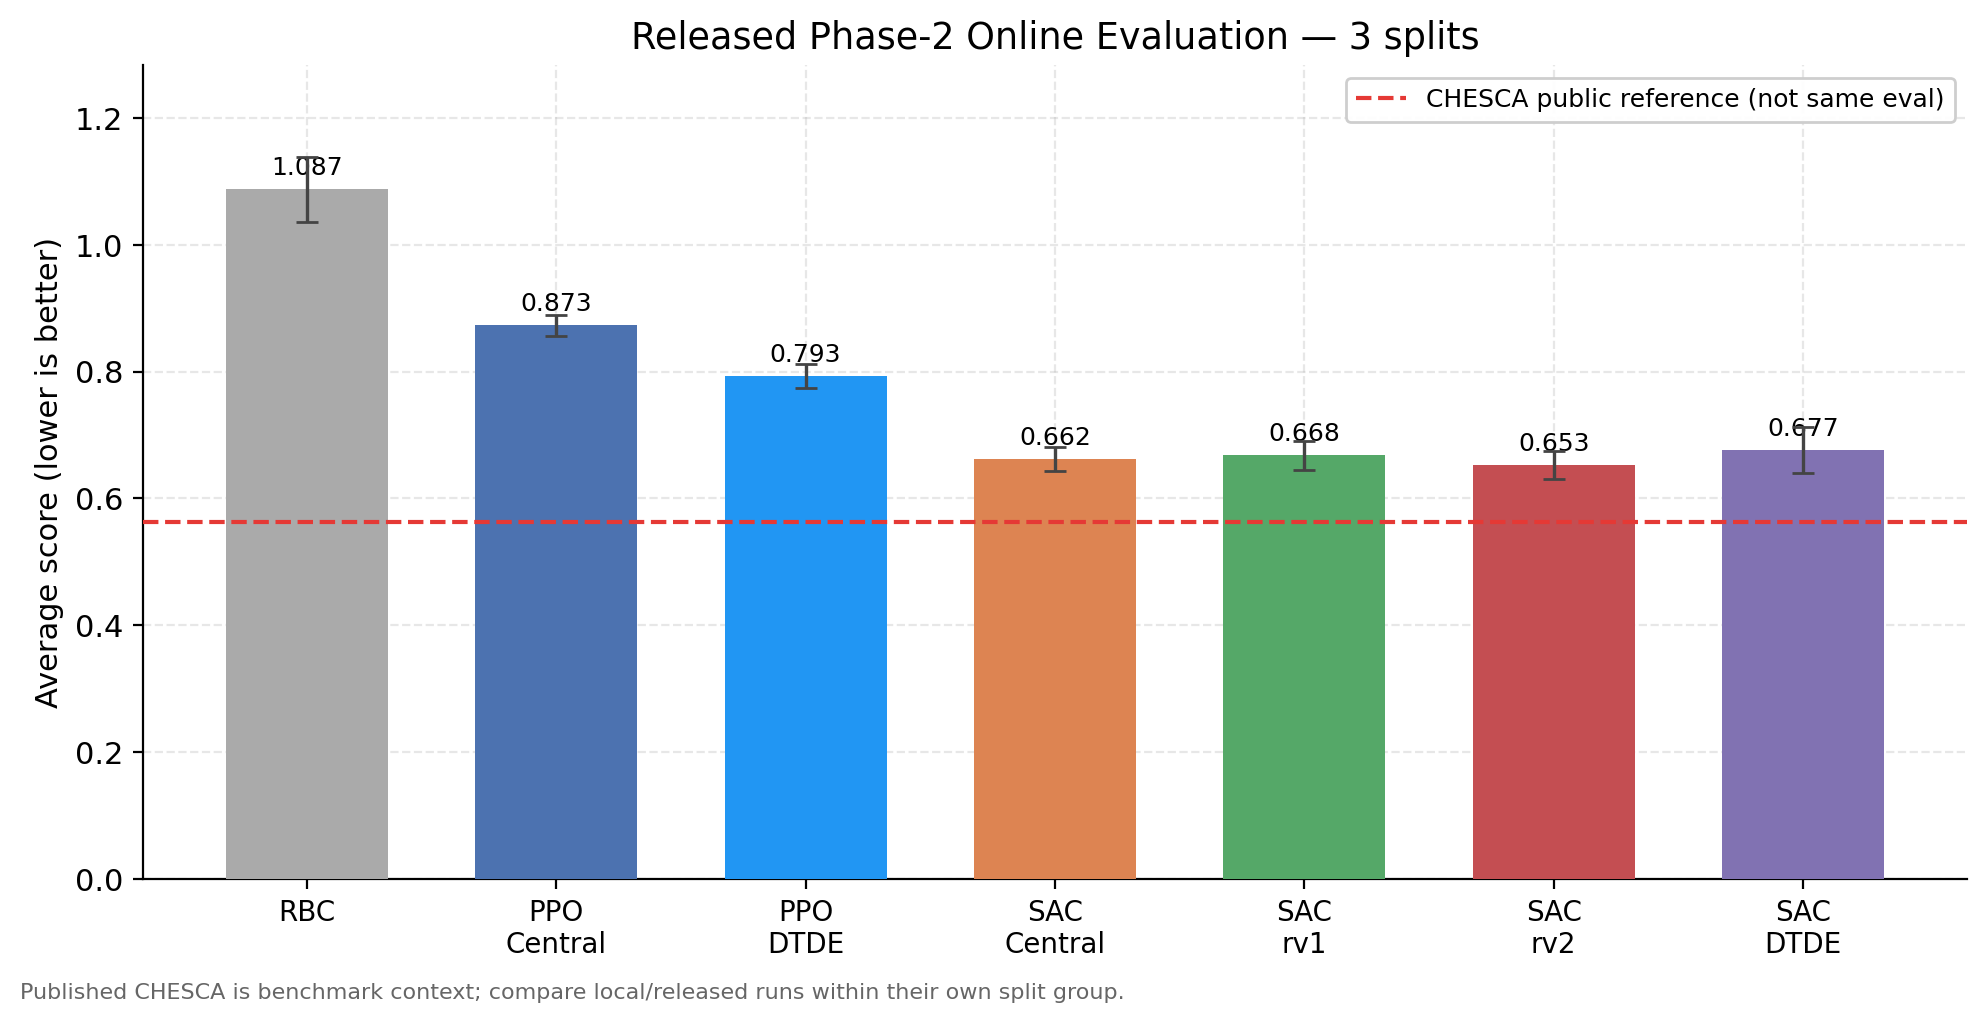
\includegraphics[width=\linewidth]{figures/cross_split_comparison.png}
    \caption{Released phase-2 comparison. Bars aggregate three held-out 3-building splits; error bars show 95\% confidence intervals over evaluation jobs. SAC \texttt{reward\_v2} is the best single-checkpoint policy.}
    \label{fig:cross_split}
\end{figure}

\paragraph{Checkpoint ensemble result.} Averaging saved centralized SAC checkpoints improves same-topology held-out performance beyond the best individual checkpoint. The strongest variant is the all-central mean-action ensemble, which reaches a released phase-2 mean of 0.616, improving on the best single-checkpoint SAC \texttt{reward\_v2} mean of 0.653 by 0.036 absolute score units. Its per-split scores are 0.660, 0.636, and 0.553. Other ensemble variants cluster tightly between 0.617 and 0.619, suggesting that ensembling reduces checkpoint-specific variance but does not change the broader conclusion: centralized SAC improves same-topology phase-2 performance, while portability still requires shared-DTDE control.

\begin{table}[ht]
\centering
\small
\begin{tabular}{lcc}
\toprule
\textbf{SAC ensemble variant} & \textbf{Public dev} & \textbf{Phase-2 mean} \\
\midrule
All-central mean action & 0.526 & 0.616 \\
Critic-guided refinement & 0.522 & 0.617 \\
Central-baseline mean action & 0.543 & 0.617 \\
Temporal-bootstrap ensemble & 0.533 & 0.618 \\
Weighted public-dev ensemble & 0.514 & 0.619 \\
\bottomrule
\end{tabular}
\caption{SAC checkpoint-ensemble ablations on 3-building phase-2 splits. Lower is better.}
\label{tab:sac_ensemble}
\end{table}

\begin{figure}[ht]
    \centering
    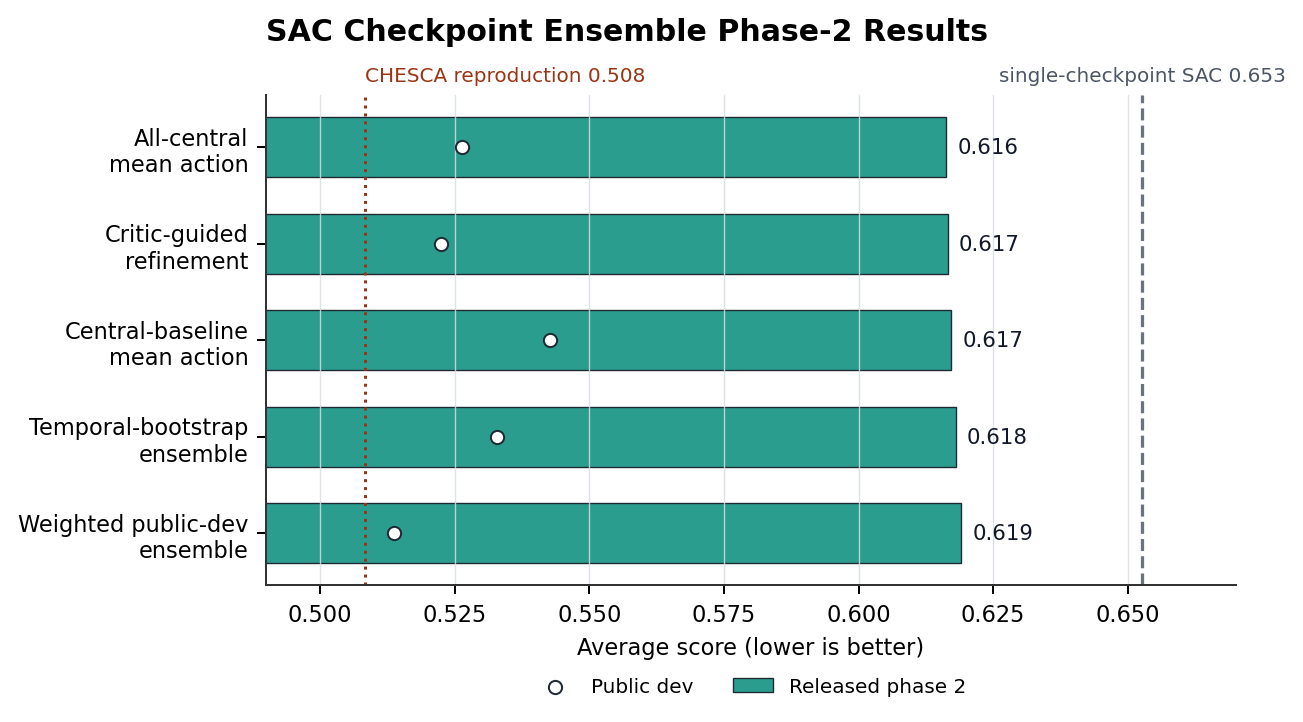
\includegraphics[width=\linewidth]{figures/sac_ensemble_phase2.png}
    \caption{Released phase-2 SAC checkpoint ensembles. Bars show held-out means over three splits; points show public-dev scores. Reference lines mark single-checkpoint SAC and CHESCA optimization context.}
    \label{fig:sac_ensemble}
\end{figure}

\paragraph{Cross-size generalization to phase-3.} The released phase-3 splits expand the cluster from 3 to 6 buildings, providing the strictest generalization test. Centralized policies fail outright here: feeding a 6-building observation to a 3-building checkpoint is a shape mismatch, not a performance question. Among portable methods, SAC shared-DTDE achieves 0.774 (mean over three splits, nine seed $\times$ split evaluation jobs), compared to 0.843 for PPO shared-DTDE and 1.114 for RBC. Shared-DTDE treats buildings as repeated instances of the same local control problem, so the same forward pass applies independently to each building's observation and no architectural change is needed. SAC-DTDE's advantage over PPO-DTDE persists on phase-3, likely because additional buildings supply more diverse per-building replay data for the off-policy learner.

\begin{figure}[ht]
    \centering
    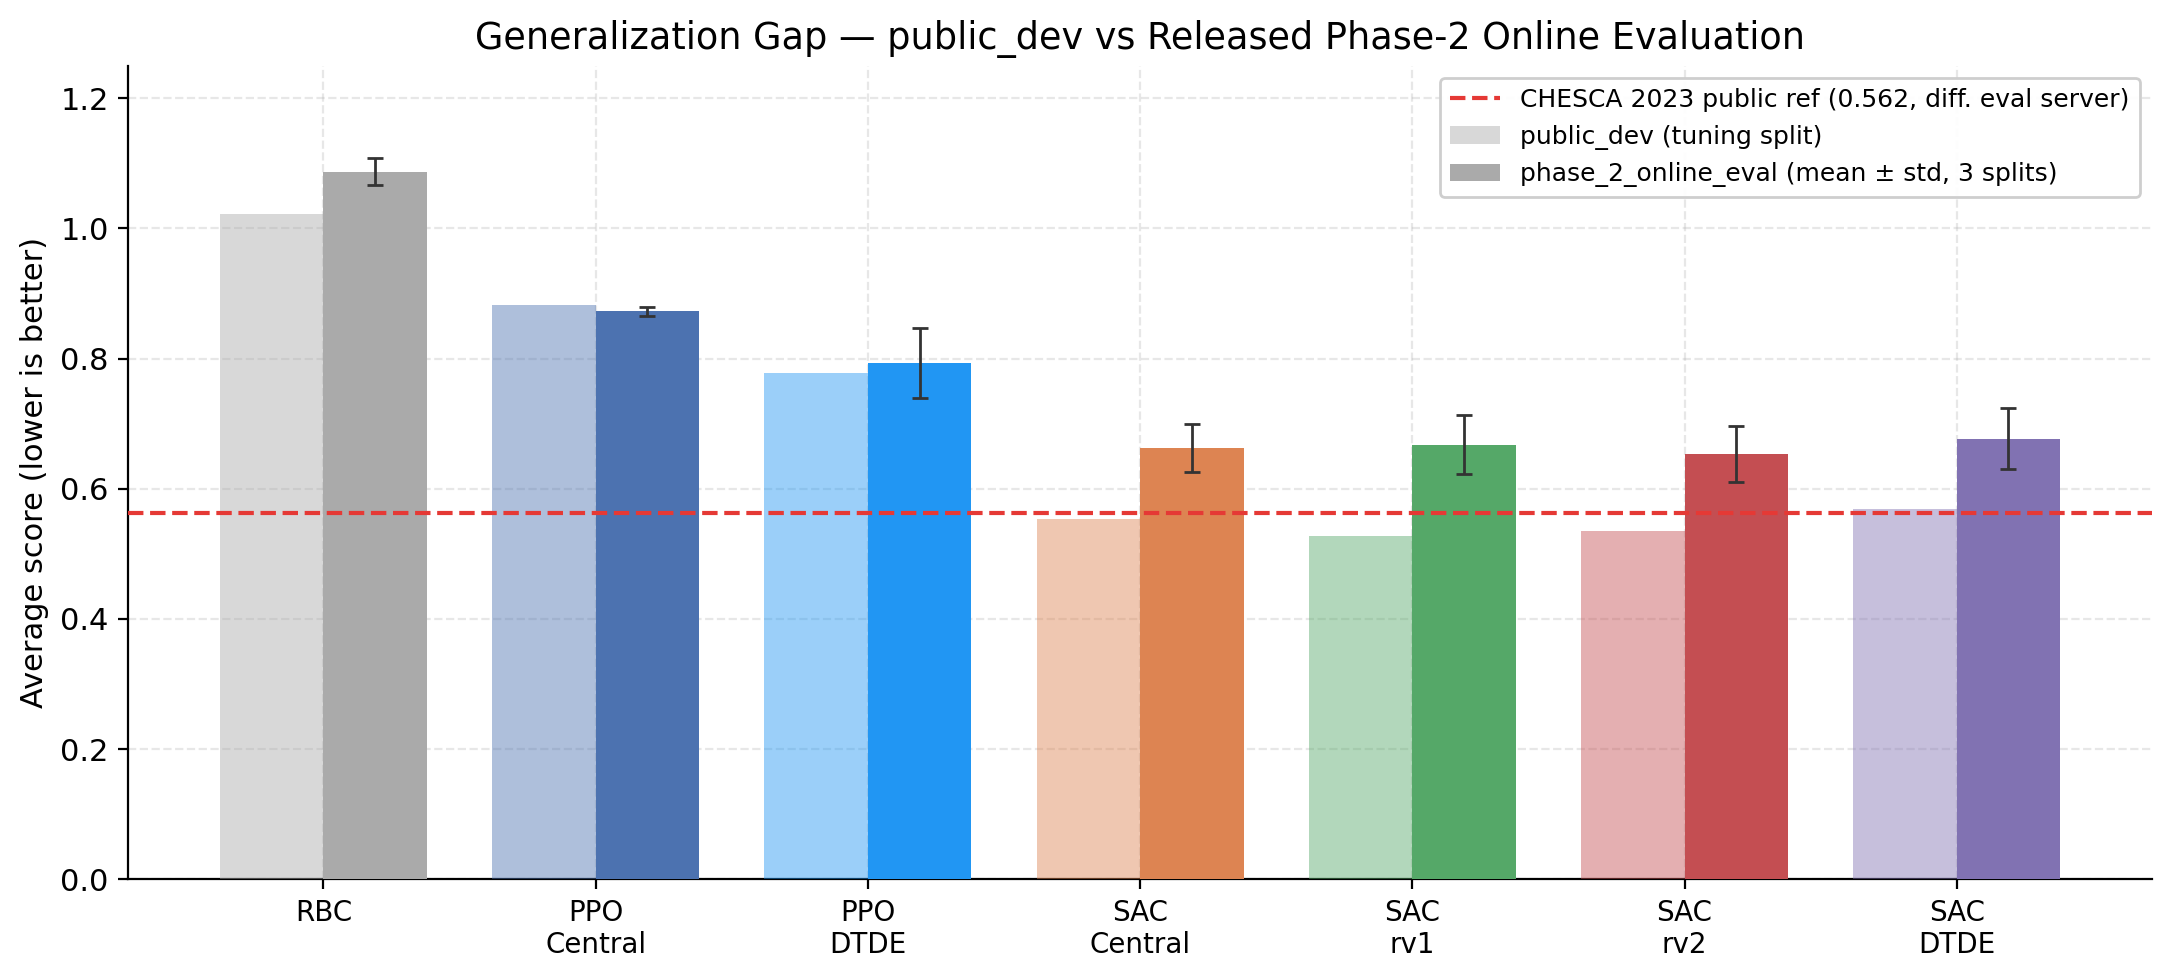
\includegraphics[width=\linewidth]{figures/generalization_gap.png}
    \caption{Local vs.\ released phase-2 scores by method. SAC variants retain the best held-out scores; PPO shared-DTDE has a smaller gap but a weaker absolute score.}
    \label{fig:gen_gap}
\end{figure}

\paragraph{KPI breakdown.} Figure~\ref{fig:kpi} disaggregates the local composite score into its constituent KPI groups. The dominant improvement comes from thermal discomfort, which carries weight 0.30 in the scoring formula. The best SAC variants reduce the discomfort proportion from 0.944 (RBC) to below 0.020. This single term explains why all RL policies beat RBC substantially even when cost and carbon reductions differ. Carbon emissions and electricity cost both fall by roughly 55\%. The main remaining weakness is thermal-resilience loss (\texttt{one\_minus\_thermal\_resilience}). SAC centralized \texttt{reward\_v1} improves this term relative to RBC (0.290 vs.\ 0.454), but it remains a visible contributor. Optimization-based methods such as CHESCA and MPC have a structural advantage here because they can plan over storage and resilience constraints with an explicit horizon rather than learning tradeoffs only from sampled trajectories.

\begin{figure}[ht]
    \centering
    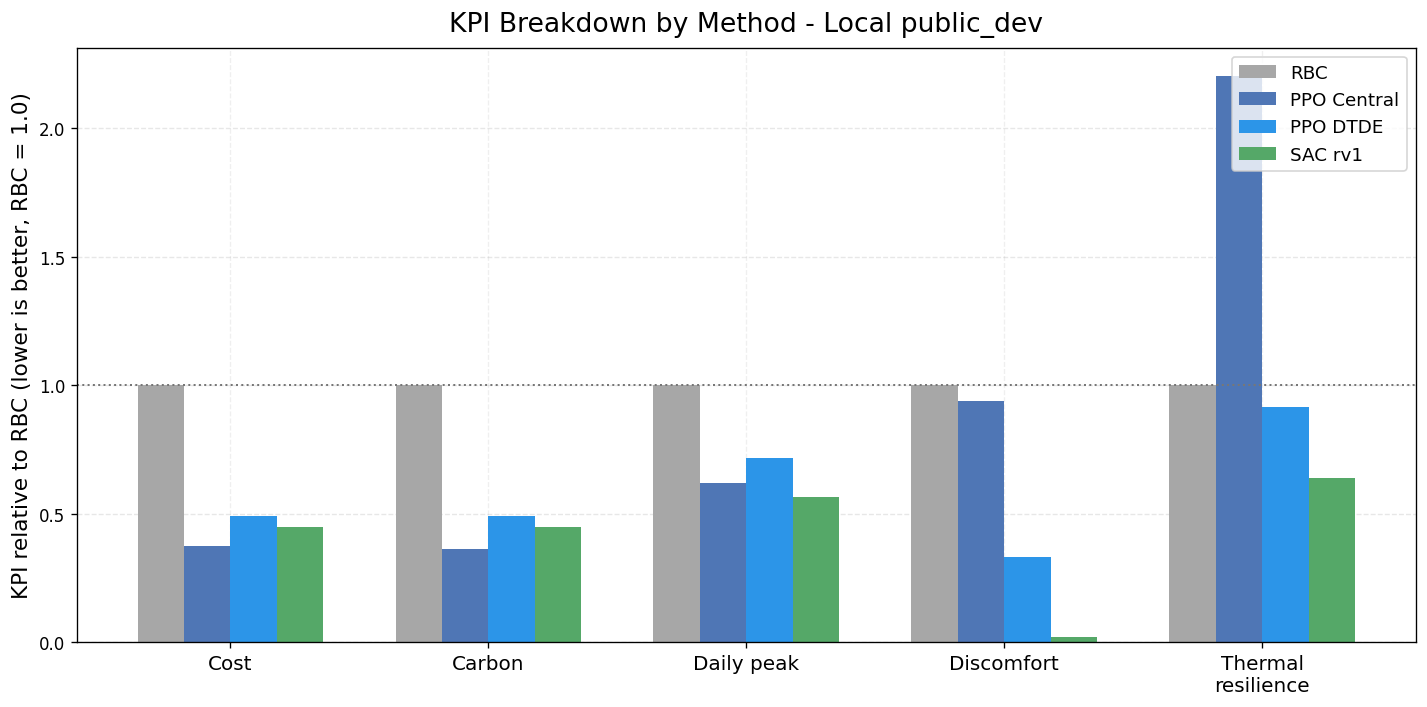
\includegraphics[width=\linewidth]{figures/kpi_breakdown.png}
    \caption{KPI breakdown on local \texttt{public\_dev}, normalized relative to RBC (RBC $=1$; lower is better). RL improves thermal discomfort most sharply; thermal-resilience loss remains the main residual weakness.}
    \label{fig:kpi}
\end{figure}

\paragraph{Reward design ablation.} Among centralized SAC variants, the baseline reward (\texttt{rv0}) is weakest locally at 0.554. \texttt{reward\_v1}, which mirrors the official 8-term weighting, achieves the best local mean at 0.527. \texttt{reward\_v2} is slightly worse locally (0.536) but leads on phase-2 (0.653 vs.\ 0.668 for \texttt{rv1}), supporting the hypothesis that smoothness penalties reduce local overfitting. The full KPI breakdown is in Table~\ref{tab:sac_ablation} in the Appendix. The most notable pattern is that the baseline reward produces the best thermal-resilience-loss score (0.166 vs.\ 0.290--0.338), possibly because explicit KPI weighting redirects battery capacity away from resilience-improving behavior.

\paragraph{PPO training diagnostic.} Figure~\ref{fig:ppo_curve} shows the centralized PPO baseline training curve used as a learning sanity check. Mean episode reward rises rapidly early in training and then flattens, indicating that PPO learns a nontrivial policy before final evaluation. This figure is not the multiseed shared-DTDE learning-rate sweep; final PPO comparisons come from Tables~\ref{tab:local} and~\ref{tab:final_matrix}.

\begin{figure}[ht]
    \centering
    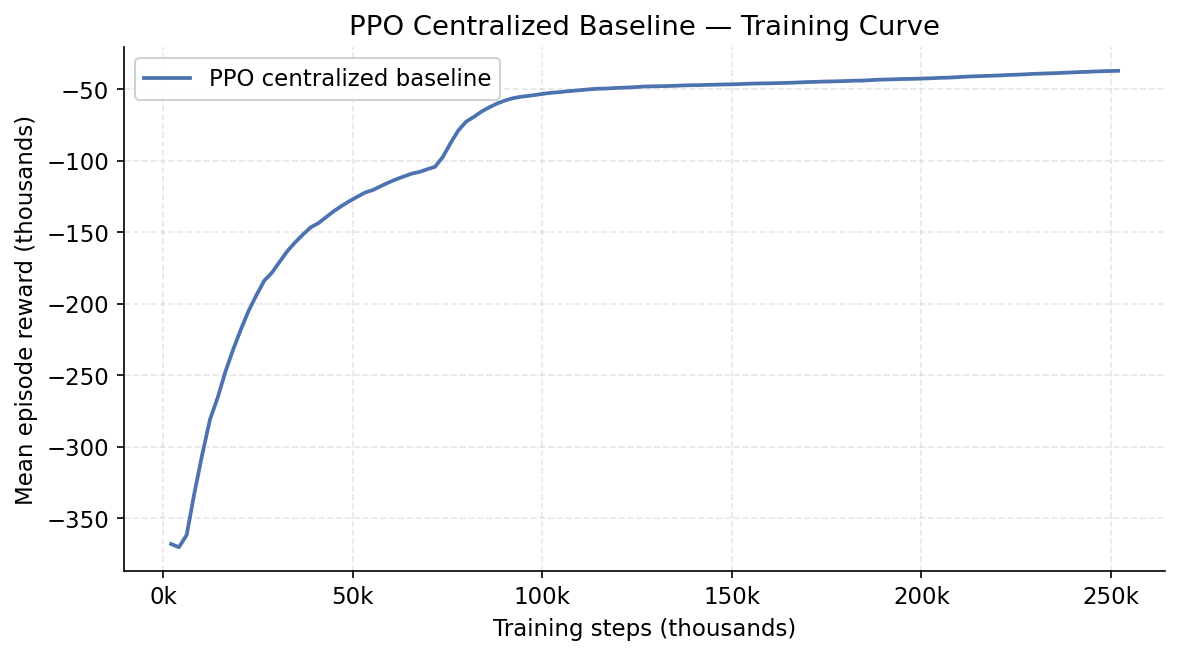
\includegraphics[width=0.75\linewidth]{figures/ppo_training_curve.png}
    \caption{Centralized PPO baseline training curve. Mean episode reward improves early and plateaus; final comparisons use the multiseed evaluation scores in Tables~\ref{tab:local} and~\ref{tab:final_matrix}.}
    \label{fig:ppo_curve}
\end{figure}

\section{Discussion and Limitations}\label{sec:discussion}

The results above establish that architectural portability is the binding constraint for real deployment, SAC substantially outperforms PPO in this continuous-control setting, and RL baselines can close much of the gap to RBC through careful reward design and evaluation discipline, but remain below published optimization-based winners. We discuss these findings and limitations below.

\paragraph{Architectural portability is the primary design axis.} The cleanest finding is architectural rather than algorithmic. If deployment may involve a different number of buildings than training, a centralized policy is incompatible by construction, while a shared-DTDE policy transfers without any network changes. On 3-building splits, centralized SAC slightly outperforms shared-DTDE SAC; the cost of decentralization is a small local score penalty of about 0.04 absolute score units. Phase-3 reverses the ordering entirely. Shared-DTDE is the only topology that can produce a score at all (0.774 for SAC-DTDE vs.\ N/A for SAC centralized). Because real neighborhoods vary in size and a deployed system may be extended over time, practical RL controllers for building energy management should account for this portability constraint at design time rather than treating it as an afterthought.

\paragraph{SAC substantially outperforms PPO for this domain.} Across topologies and splits, SAC variants consistently produce lower composite scores than comparable PPO variants, though the absolute gap depends on the comparison: it is about 0.07--0.12 absolute score units in the shared-controller released and final-sweep matrices, and much larger in the local centralized baseline comparison. The most likely explanation is sample efficiency. SAC reuses historical transitions through off-policy replay, and entropy regularization reduces sensitivity to reward scaling. PPO is simpler to implement because it avoids replay buffers and target networks, but that simplicity does not translate to better performance in continuous battery control where replay is directly beneficial.

\paragraph{TD3 is useful but not a replacement for SAC.} The final sweeps make TD3 a credible additional baseline rather than just an implementation exercise. It gives the best broad-sweep phase-3 transfer score, which suggests deterministic off-policy control can exploit the shared topology when the learning rate is tuned well. However, SAC remains stronger in the targeted released-all matrix and is less brittle across nearby learning rates, so the safest final claim is that SAC is the best overall learned controller while TD3 is competitive on transfer.

\paragraph{Reward design matters within SAC.} The gap between the SAC baseline and \texttt{reward\_v1} (0.554 vs.\ 0.527 locally) shows that training on the official scoring objective outperforms training on a proxy. The smoothness penalties in \texttt{reward\_v2} trade a small local regression for better phase-2 generalization. Large SoC swings and repeated sign flips become costly even if they improve a short local trajectory, and this behavioral regularization transfers better when weather and demand traces change. For deployment on new buildings, \texttt{reward\_v2} is therefore the more robust choice. An important practical implication is that the reward design decision is inseparable from the evaluation protocol. If we had only measured performance on the local \texttt{public\_dev} split, we would have selected \texttt{rv1} as the best reward and missed the fact that \texttt{rv2} generalizes better. This underscores the value of held-out evaluation even for design choices that appear secondary to algorithm selection.

\paragraph{Comparison to optimization-based methods.} CHESCA achieved 0.562 on the official 2023 public leaderboard \citep{pinto2024citylearn}, better than our best SAC-only phase-2 result of 0.616. This is benchmark context, not a head-to-head comparison, because our phase-2 results use the subsequently released evaluation datasets rather than the original competition server. In our released phase-2 reproduction harness, upstream CHESCA scores 0.508, and a CHESCA residual plus SAC action blend reaches 0.501; those rows are optimization and hybrid context rather than standalone learned-controller evidence. Substantively, CHESCA and the HKUST solution \citep{zheng2025optimizing} use hierarchy to separate building-level and community-level objectives, giving them a natural way to reserve storage for future events and enforce resilience constraints. Our shared-DTDE policies gain portability by treating buildings as independent instances, but they give up the community-level optimization layer. A natural next step is a hybrid controller that combines the portability of shared-DTDE with an MPC or optimization layer that enforces aggregate grid and resilience constraints.

\paragraph{Limitations.}
\begin{itemize}
    \item Single tuning split. All reward variants and hyperparameters were selected on the local \texttt{public\_dev} split. A stronger protocol would reserve a separate validation split to reduce the risk of overfitting design choices to one dataset.
    \item Compute constraints. SAC shared-DTDE was run with only 3 seeds in the pilot matrix, and the reward-variant ablation was not conducted for PPO due to GPU budget limits. The PPO sweep covered 10 seeds but only two learning rates; wider sweeps might yield better configurations.
    \item Confidence intervals. Our CIs aggregate evaluation jobs unless otherwise stated. Because jobs from the same released split are correlated, a split-clustered bootstrap would be a stronger uncertainty estimate for cross-split generalization claims.
    \item Final sweep selection. The PPO/SAC/TD3 matrix uses three seeds per hyperparameter cell and selects the best setting within each algorithm/evaluation group. This is useful for robustness evidence, but it is not a blind leaderboard protocol.
    \item Checkpoint ensembling is same-topology only. The SAC ensemble improves released phase-2 performance, but it uses centralized three-building checkpoints and does not change the phase-3 portability result.
    \item Centralized policies not portable. The centralized SAC variants, which achieve the best local scores, cannot be evaluated on phase-3 (6-building) splits. Generalization claims for centralized SAC are necessarily limited to same-topology held-out sets.
    \item No forecast model. We use only the short-horizon forecasts provided by the environment. A learned demand-prediction module could improve policy quality and is a common component of strong model-predictive baselines.
    \item CHESCA comparison is indirect. The 0.562 CHESCA reference is from the competition paper \citep{pinto2024citylearn} and was scored on a hidden split via an evaluation server that is no longer publicly accessible, making a direct numerical comparison impossible.
\end{itemize}

{\footnotesize
% \paragraph{Acknowledgements.} We thank XXX.

\bibliographystyle{apalike}
\bibliography{references}
}

\section*{Appendix}

\paragraph{Per-split generalization table.}

Table~\ref{tab:cross_split} reports the per-split composite scores used in Figure~\ref{fig:per_split}. Entries marked ``---'' indicate that a method cannot execute on that split (centralized policies on phase-3) or that results were not collected.

\begin{table}[ht]
\centering
\small
\begin{tabular}{lccccccc}
\toprule
\textbf{Method} & \textbf{public\_dev} & \textbf{p2\_e1} & \textbf{p2\_e2} & \textbf{p2\_e3} & \textbf{p3\_1} & \textbf{p3\_2} & \textbf{p3\_3} \\
\midrule
RBC                & 1.023 & 1.109 & 1.085 & 1.068 & 1.117 & 1.124 & 1.100 \\
PPO Central        & 0.883 & 0.881 & 0.868 & 0.870 & --- & --- & --- \\
PPO DTDE           & 0.777 & 0.829 & 0.813 & 0.738 & 0.846 & 0.844 & 0.840 \\
SAC Central        & 0.554 & 0.684 & 0.687 & 0.615 & --- & --- & --- \\
SAC \texttt{rv1}   & 0.527 & 0.707 & 0.686 & 0.611 & --- & --- & --- \\
SAC \texttt{rv2}   & 0.536 & 0.691 & 0.670 & 0.597 & --- & --- & --- \\
SAC ensemble       & 0.526 & 0.660 & 0.636 & 0.553 & --- & --- & --- \\
SAC DTDE           & 0.569 & 0.715 & 0.700 & 0.615 & 0.786 & 0.762 & 0.775 \\
\midrule
CHESCA (ref.)      & --- & 0.562 & --- & --- & --- & --- & --- \\
\bottomrule
\end{tabular}
\caption{Per-split composite scores ($\downarrow$ better). Phase-2 columns are 3-building released splits; phase-3 columns are 6-building released splits. CHESCA is the 2023 leaderboard reference from \citet{pinto2024citylearn}.}
\label{tab:cross_split}
\end{table}

\paragraph{SAC reward-variant ablation detail.}

Table~\ref{tab:sac_ablation} extends the local SAC comparison with KPI-level columns. All SAC variants reduce thermal discomfort from the RBC level of 0.944 to near zero ($\leq 0.020$), consistent with the 0.30 weight on this term. The SAC baseline achieves a similar reduction despite not explicitly weighting discomfort, suggesting that the net-consumption proxy also indirectly rewards occupant comfort. Differences across variants are most visible in thermal-resilience loss (0.166 vs.\ 0.290--0.338), where the baseline reward outperforms the shaped variants.

\begin{table}[ht]
\centering
\small
\begin{tabular}{lccccc}
\toprule
\textbf{Variant} & \textbf{Score} & \textbf{Cost} & \textbf{Carbon} & \textbf{Discomfort} & \textbf{1$-$Resilience} \\
\midrule
SAC baseline (\texttt{rv0}) & 0.554 & 0.888 & 0.904 & 0.012 & 0.166 \\
SAC \texttt{rv1}            & 0.527 & 0.823 & 0.848 & 0.019 & 0.290 \\
SAC \texttt{rv2}            & 0.536 & 0.811 & 0.836 & 0.020 & 0.310 \\
SAC shared-DTDE \texttt{rv2} & 0.569 & 0.809 & 0.829 & 0.023 & 0.338 \\
\midrule
Local RBC                   & 1.023 & 1.839 & 1.890 & 0.944 & 0.454 \\
\bottomrule
\end{tabular}
\caption{SAC reward-variant ablation on local \texttt{public\_dev}. KPI columns are seed-averaged means; lower is better.}
\label{tab:sac_ablation}
\end{table}

\end{document}
